\section{Get In Touch With Services}

\subsection{Casanova (70p)}
My service is running on \texttt{kenobi.hackingarena.com}, port \texttt{9393}. My name is Casanova (username: \texttt{casanova}). I have a huge problem. One of my exgirlfriends somehow figured out my password and want to realese all details about my affairs. How she figured it out??? I was so cautios. Ok, I'm using the same password everywhere, but I never had any incident (except for this emberassing Ashley Madison case). I hope you cannot login.

\textbf{Solution:}\\
I started by connecting to the service with netcat, and got the following output:

\begin{center}
    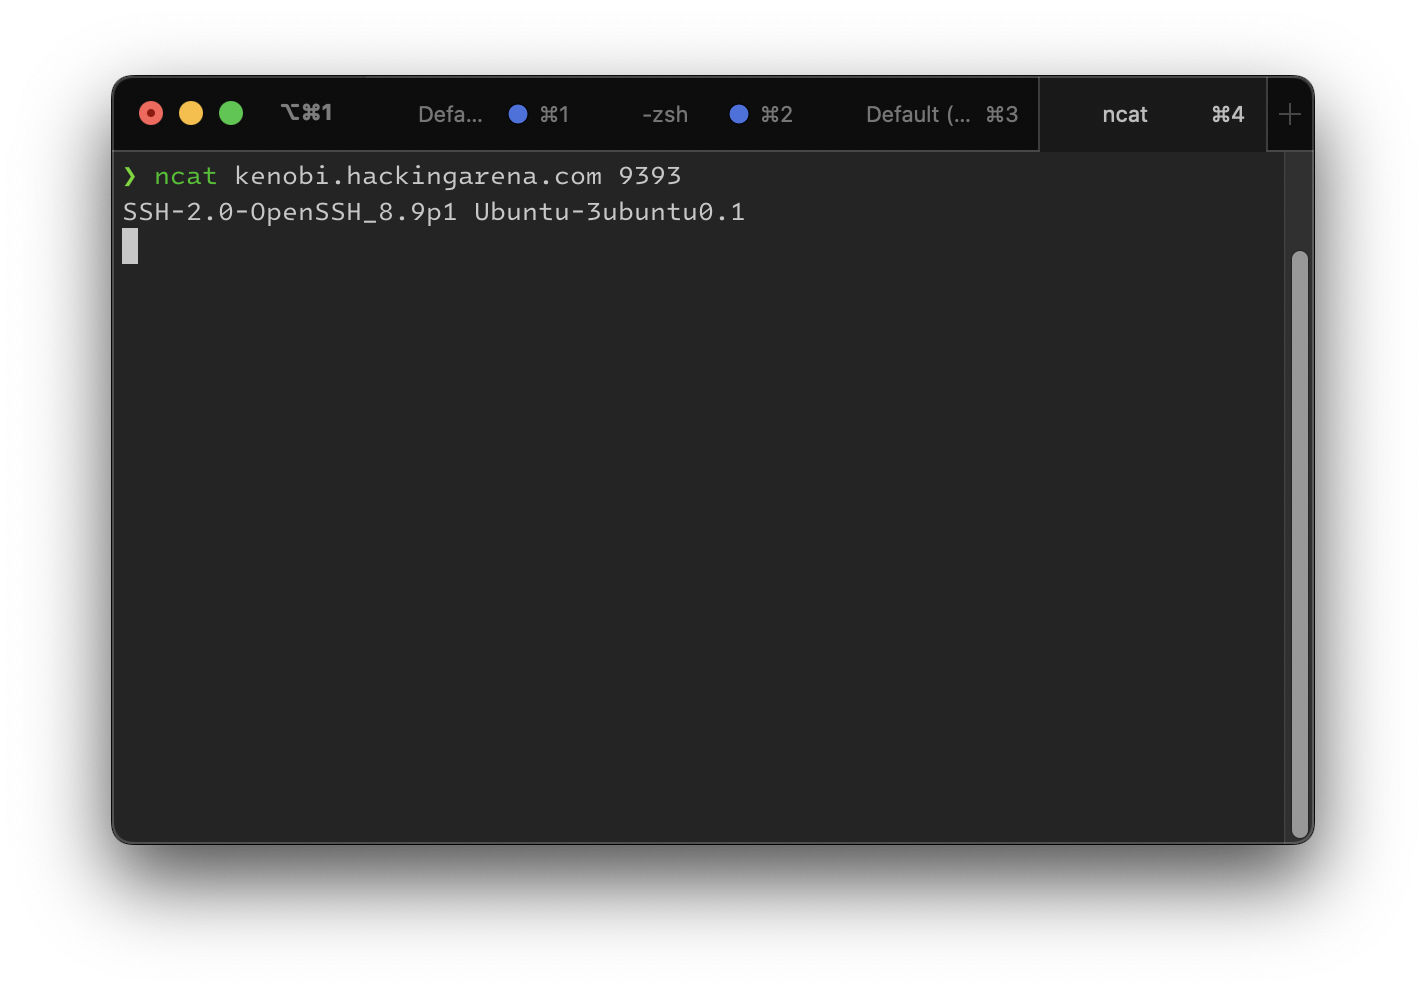
\includegraphics[width=15cm]{img/Get in touch with services/Casanova/Skjermbilde 2023-10-27 kl. 09.04.00.png}
\end{center}

That told me that an ssh service was running on the instance. I then figured the <<Ashley Madison case>> was a hint to a password breach, so i searched for it and found the top 100 passwords from the breach. I put the 100 passwords in a file called \texttt{passwrd.txt} and used hydra to brute force the password for the user \texttt{casanova} on the ssh service as such:

\begin{center}
    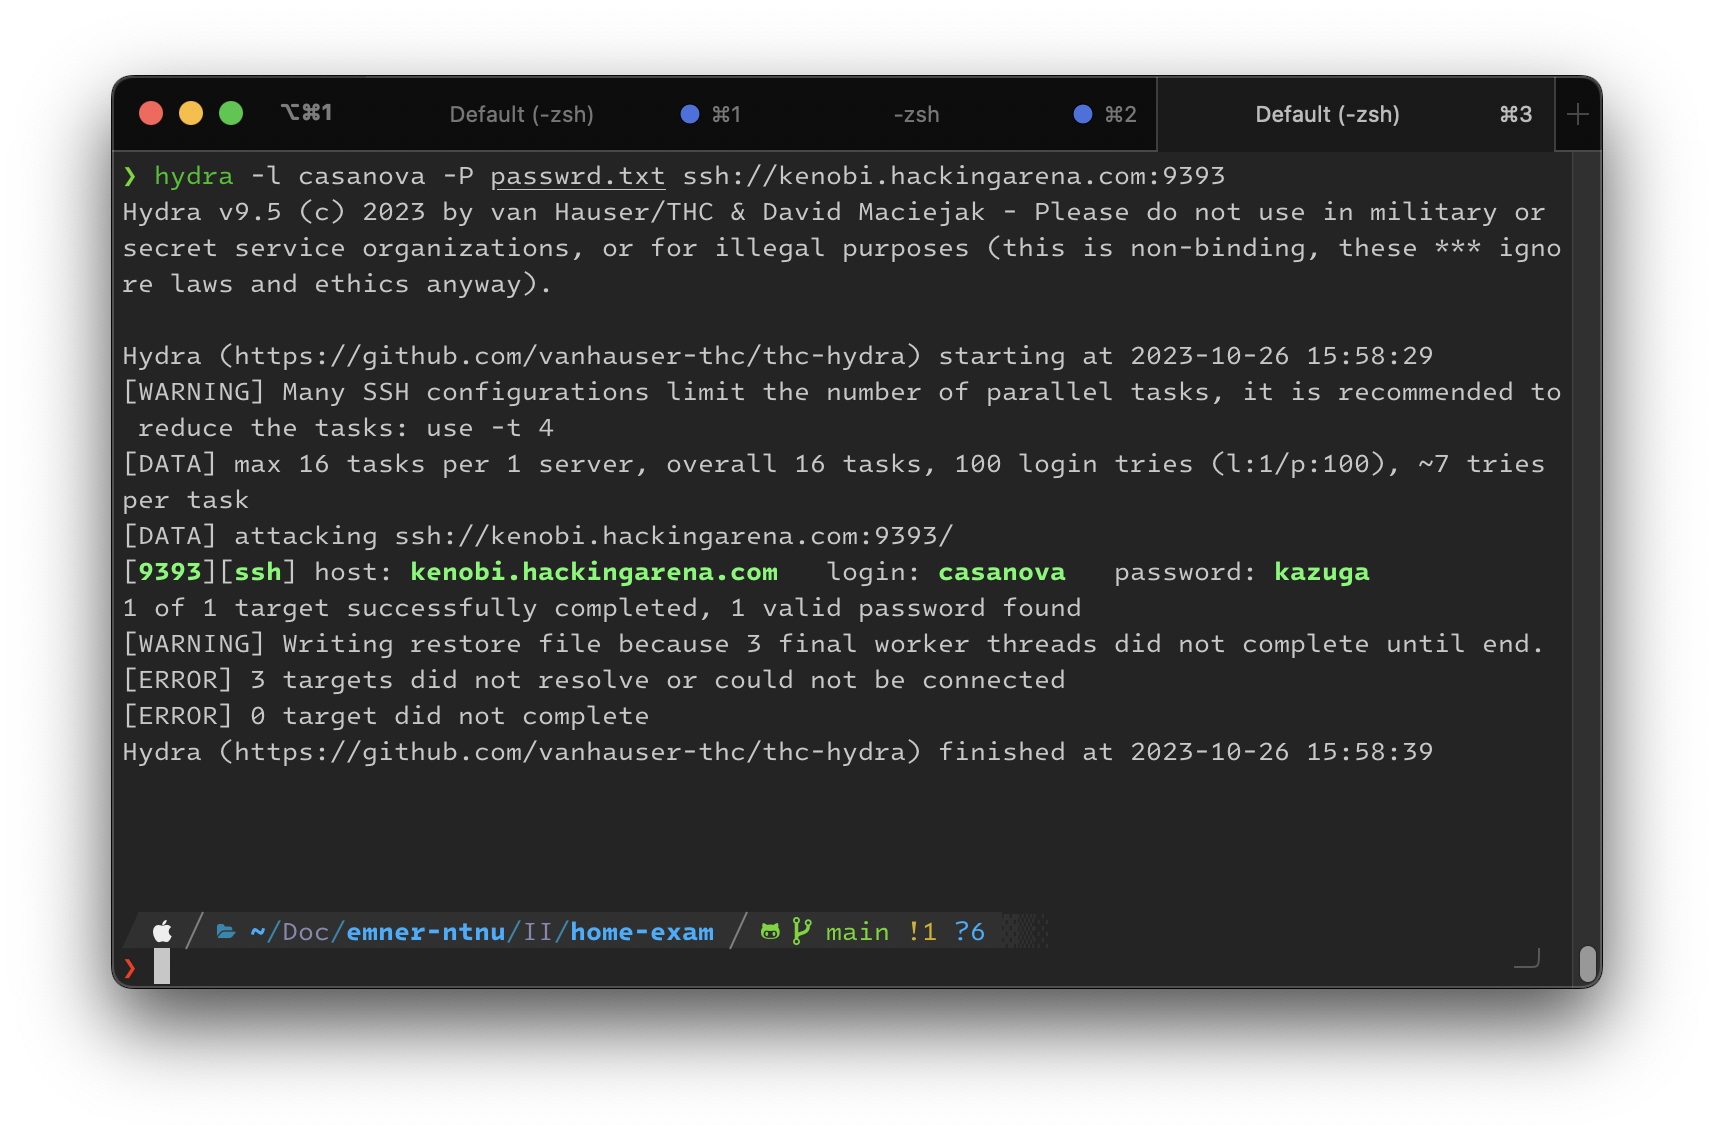
\includegraphics[width=15cm]{img/Get in touch with services/Casanova/Skjermbilde 2023-10-26 kl. 15.59.05.png}
\end{center}

I then got one hit, and the password was \texttt{kazuga}. I then connected to the service with ssh and found the flag in the home directory.

\begin{center}
    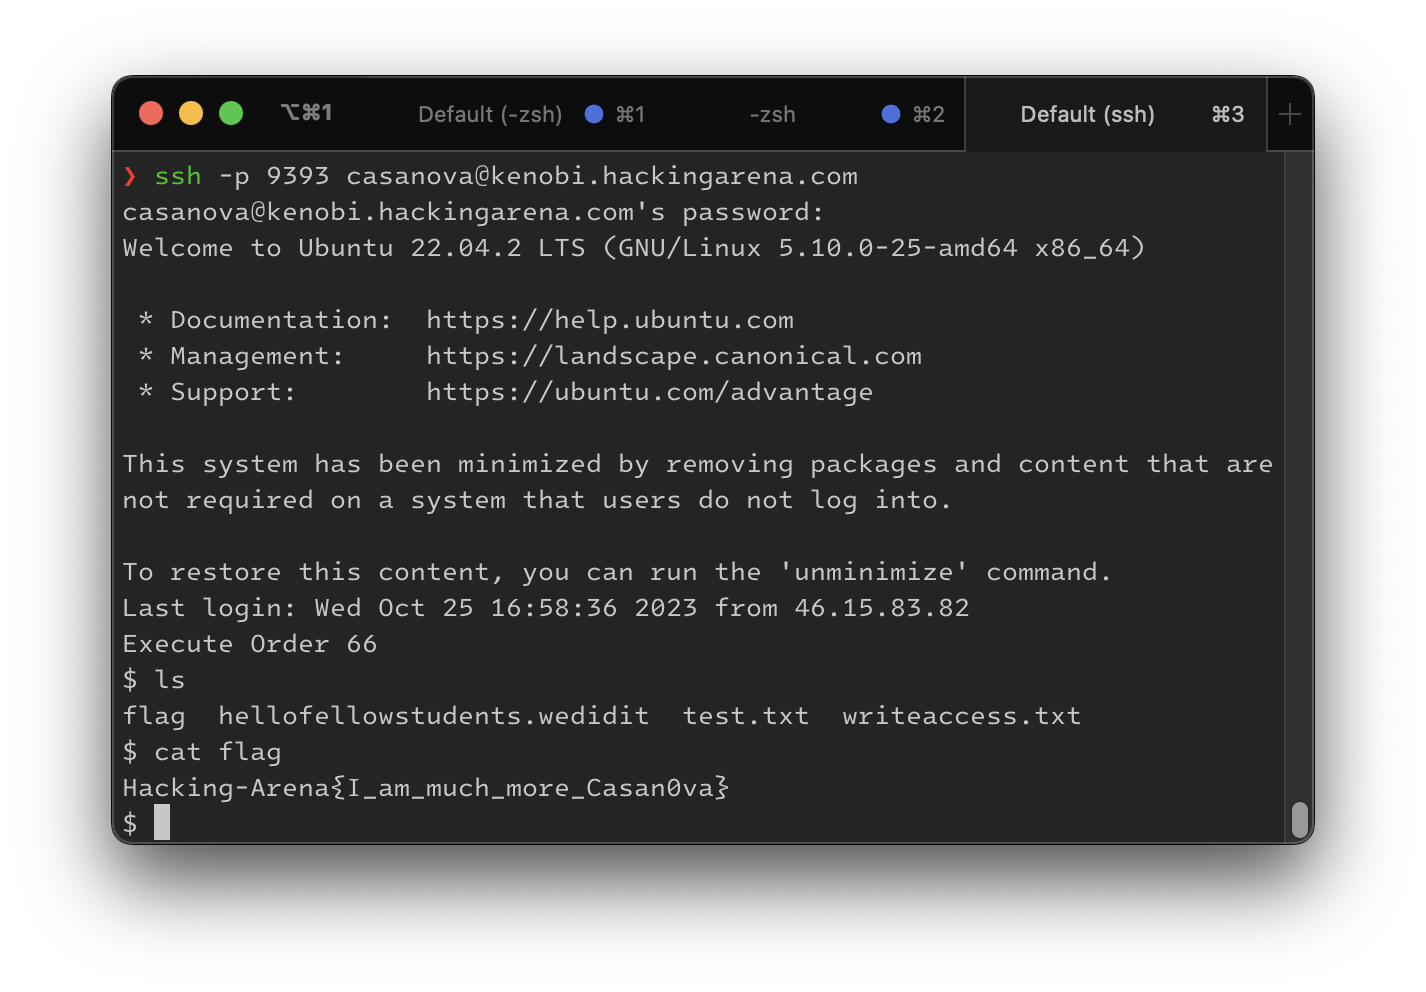
\includegraphics[width=15cm]{img/Get in touch with services/Casanova/Skjermbilde 2023-10-26 kl. 15.59.48.png}
\end{center}

The flag is: \texttt{Hacking-Arena\string{I\_am\_much\_more\_Casan0va\string}}

\newpage
\subsection{Minuteman (80p)}
A service is running on \texttt{kenobi.hackingarena.com} portrange: \texttt{7000-7500}. I hope you can find this very important flag :)

\textbf{Solution:}\\
I started by scanning the ports with nmap, and got the following output:

\begin{center}
    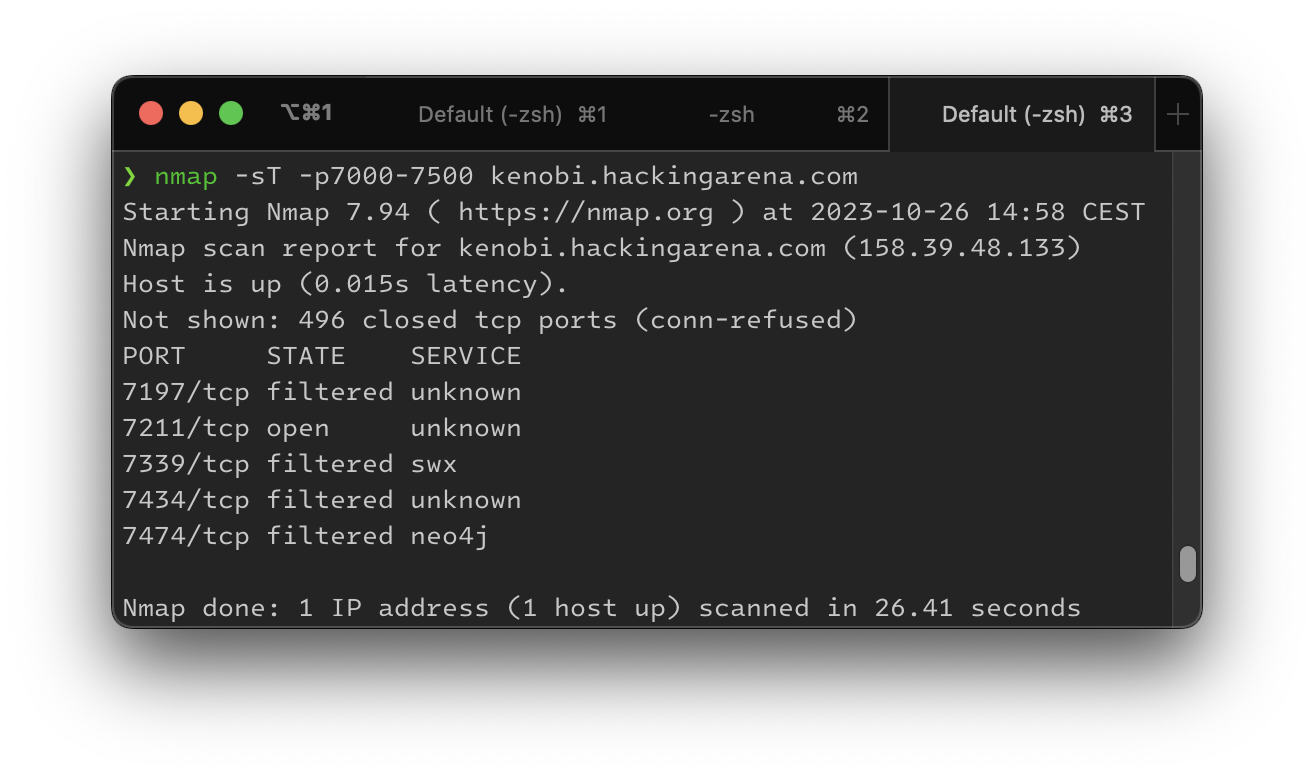
\includegraphics[width=14cm]{img/Get in touch with services/Minuteman/Skjermbilde 2023-10-26 kl. 15.14.45.png}
\end{center}

I then connected to the only open service on port 7211 with telnet, and got the following response:

\begin{center}
    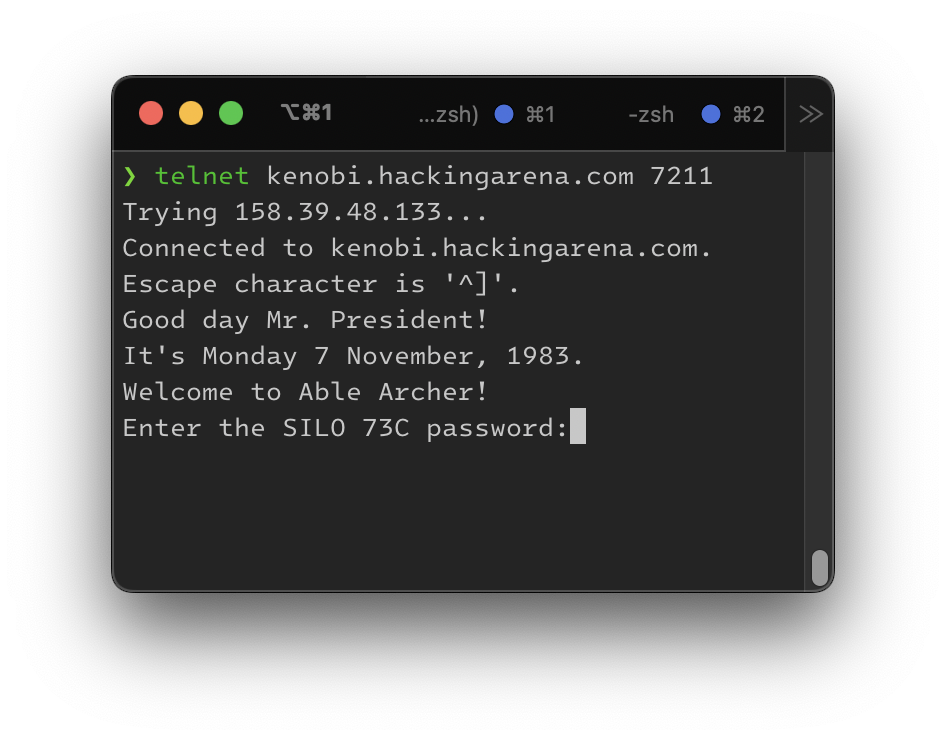
\includegraphics[width=11cm]{img/Get in touch with services/Minuteman/Skjermbilde 2023-10-27 kl. 09.30.39.png}
\end{center}

After searching for what Able Archer was, i found that it was a NATO exercise in 1983. I then found the nuclear launch codes for the exercise, which was \texttt{00000000}. I then connected to the service again with telnet, gave it the launch codes, and got the following response:

\begin{center}
    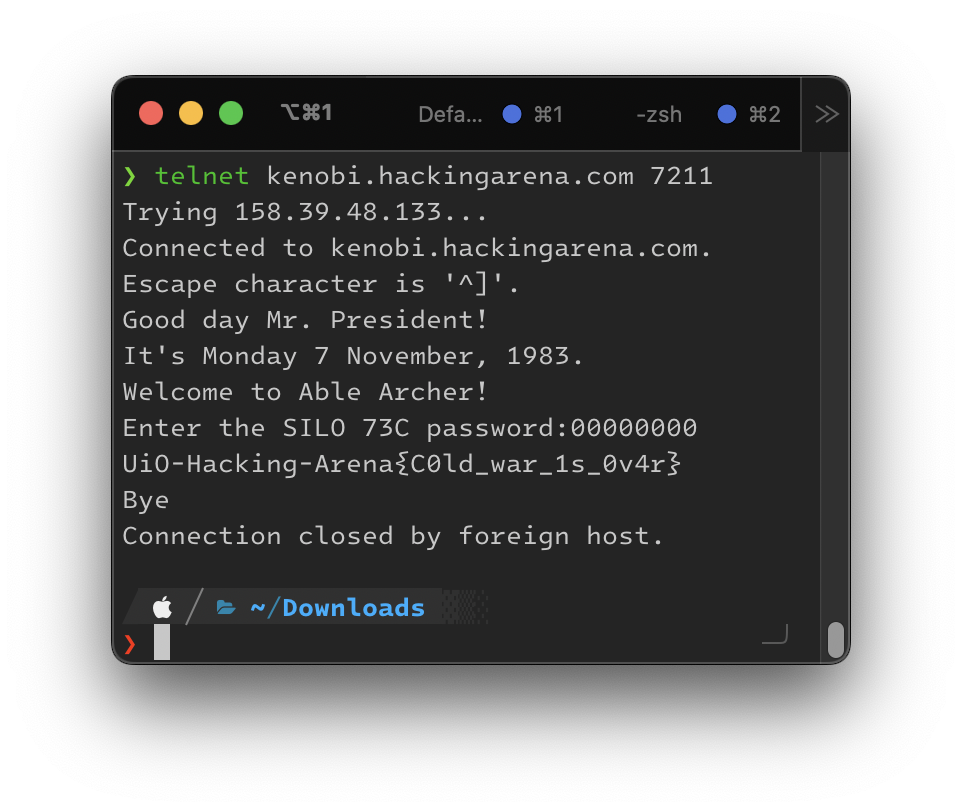
\includegraphics[width=12cm]{img/Get in touch with services/Minuteman/Skjermbilde 2023-10-26 kl. 15.13.55.png}
\end{center}

The flag was \texttt{UiO-Hacking-Arena\string{C0ld\_war\_1s\_0v4r\string}}.

\newpage
\subsection{Dark energy (90p)}
Have you already checked padawan ports? What was this on \texttt{tcp/502}? Maybe there is a flag for you. :)

\textbf{Solution:}\\
First i had to check again what service was running on port 502, and found that it was modbus.
I then downloaded a \href{https://github.com/tallakt/modbus-cli}{modbus client} and followed the README instructions and ran the command:
\texttt{modbus read -p502 padawan.hackingarena.com \%MW100 50}
which read 50 registers from the modbus server on port 502.

\begin{center}
    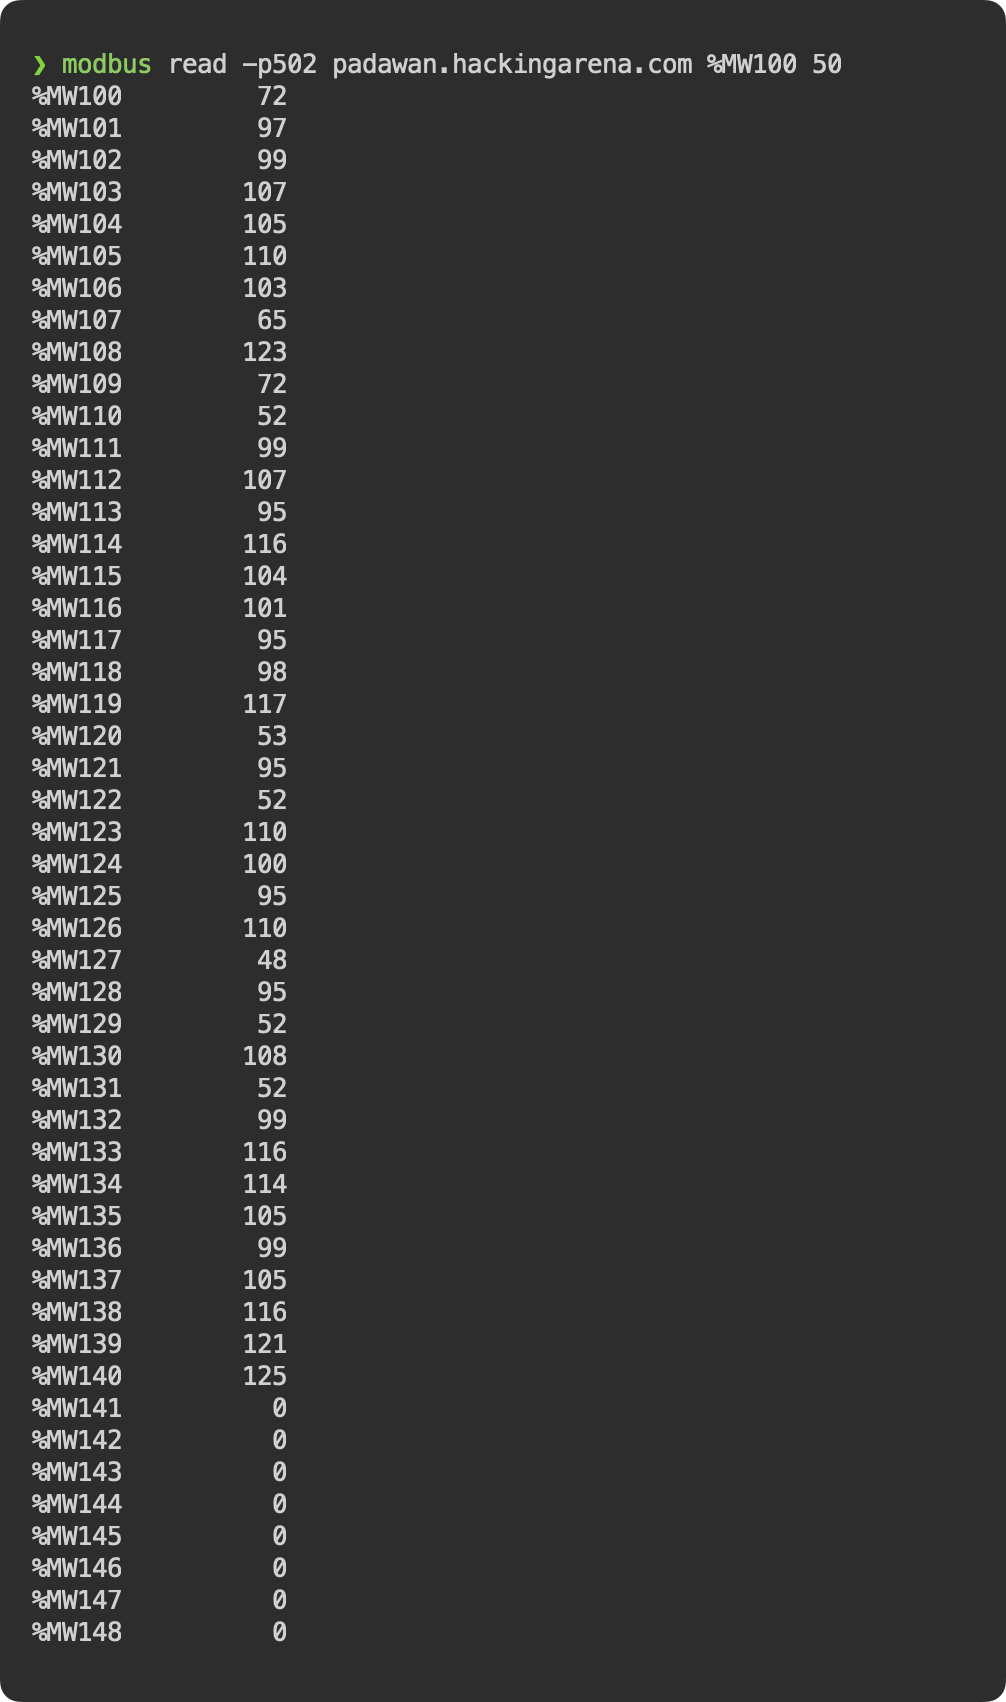
\includegraphics[width=9cm]{img/Get in touch with services/Dark energy/Screenshot 2023-11-10 at 10.38.21.png}
\end{center}

I then copied the numbers from the output and converted them from decimal to ascii, and got the following flag:
\texttt{HackingA\string{H4ck\_the\_bu5\_4nd\_n0\_4l4ctricity\string}}